\documentclass[11pt]{exam}
\usepackage{style/preamble}
\newcommand{\name}{Section 11: Panel Data}


\begin{document}
\noindent
\fbox{%
  \begin{minipage}[t]{\linewidth}
    \class, \term \hfill
    \begin{center}
      \textbf{\Large \name}
    \end{center}
    \emph{\tanames} \hfill
  \end{minipage}
}
\begingroup\small

\section{Difference-in-Differences}
\subsection{Motivation}
So far, we have only considered settings in which each unit is either treated or not treated once, and we observe a single outcome. In many applications, however, we observe the \emph{same} units repeatedly over time. In this section we focus on the case where all units start in control and, at some later time, a subset of units is exposed to the treatment. Our parameter of interest is the average treatment effect on the treated (ATT), since we care about the effect for those units that actually receive the treatment.

Because time now plays a central role, we will use $t$ to index time and reserve $Z_{it} \in \{0,1\}$ for the treatment indicator (rather than $T$, which we used earlier).

How should we conduct causal inference in this setting? Consider the simple case where treatment is first given at time $t+1$, and no unit is treated at time $t$. For a treated unit $i$, the causal effect at time $t+1$ is
\[
  \tau_{i t+1}= Y_{it+1}(1) - Y_{it+1}(0),
\]
but we only observe either $Y_{it+1} = Y_{it+1}(1)$ and $Y_{it} = Y_{it}(0)$, but not $Y_{it+1}(0)$. 

Thus, a first idea is to compare the same unit \emph{before} and \emph{after} treatment,
\[
  Y_{it+1} - Y_{it}.
\]
This is illustrated in the left panel of Figure~\ref{fig:naive_temp}. However, for a treated unit $i$, this implicitly assumes $Y_{it}(0) = Y_{it+1}(0),$
i.e., that the untreated outcome would not change over time. This is often unrealistic, as it fails to account for changes over time.

A second idea is to use units that remain in the control group, as in the right panel of Figure~\ref{fig:naive_temp}. We could compare the treated unit $i$ to some control unit $j$ at time $t+1$,
\[
  Y_{it+1}(1) - Y_{jt+1}(0).
\]
Now we are comparing different units at the same time, which assumes $ Y_{it+1}(0) = Y_{jt+1}(0)$. This is also hard to justify, as it fails to account for systematic difference between the treated and control (recall that treatment is not randomized).

In what follows, we develop a method called \emph{difference-in-differences} that aims to estimate $Y_{it+1}(1) - Y_{it+1}(0)$ (more precisely, its average)
more credibly by combining the time comparison and the cross-sectional comparison. The key assumption is that units remaining in control satisfy the \emph{parallel trends} assumption, illustrated in Figure~\ref{fig:parallel_trend}.



% So far, we have only considered the case where units receive treatment exposure (or not) and their outcome is recorded. However, in many application we have repeated measurements of the same unit over time. We focus on the setting where all units start in control and at a later time point some units are given the treatment, while others stay in control through the entire duration. Thus, we focus on the $\ATT$, as we are interested in the effect of the treated units. Since time plays an important role, we will denote treatment with $Z$ instead of $T$, which we use to index time instead.

% How should we conduct causal inference in this setting? Assume the simple case where treatment is given at time $t+1$ but none at time $t$. Focusing on a single unit, we would like to compare $Y_{i{t+1}}(1) - Y_{i{t+1}}(0)$. However, we never observe $Y_{i{t+1}}(0)$.
% A simple solution would be to compare the same unit \emph{before} and \emph{after} the treatment was given, i.e. $Y_{i{t+1}} - Y_{it}$. This is illustrated in the left plot of Figure~\ref{fig:naive_temp}. However, this assumes that $Y_{it}(0) = Y_{i{t+1}(0)}$, which might not be the case, for example if the outcome follows a trend over time. 

% Another solution is to make use of units which sty in the control group, as illustrated in the right plot of Figure~\ref{fig:naive_temp}. In this case, we compare $Y_{i{t+1}}(1) - Y_{j{t+1}}(0)$ for some unit $j$ in the control group. Of course, now we don't compare the same unit and we thus assume that $Y_{i{t+1}}(0) = Y_{j{t+1}}(0)$, which seems arbitrary, even on average.

% In this section we discuss an approach to directly estimate $Y_{i{t+1}}(1) - Y_{i{t+1}}(0)$ by assuming that units in control follow the so-called \emph{parallel tend} assumption, illustrated in Figure~\ref{fig:did}.


\begin{figure}[htbp]
  \centering
  % Left: CS
  \begin{minipage}[b]{0.48\textwidth}
    \centering
    
\includegraphics[width=\textwidth]{figures/BA.pdf}
    \caption*{Before-After}
  \end{minipage}
  \hfill
  % Right: BA
  \begin{minipage}[b]{0.48\textwidth}
    \centering
    
\includegraphics[width=\textwidth]{figures/CS.pdf}
    \caption*{Cross-Sectional}
  \end{minipage}
  \caption{Taken from Kosuke Imai's lecture slides.}
  \label{fig:naive_temp}
\end{figure}

\begin{figure}[htbp]
  \centering
  \begin{tikzpicture}[
    >=latex,
    scale=2,            % <-- enlarge the whole figure
    every node/.style={font=\small}
  ]

    % Axes ----------------------------------------------------
    \draw[->] (0,0) -- (4.2,0);    % x-axis
    \draw[->] (0,0) -- (0,3.0);    % y-axis

    % Axis labels
    \node[below]        at (2,-0.2)   {Time};
    \node[rotate=90]    at (-0.2,1.5) {Average Outcome};

    % Time points
    \coordinate (t0) at (1,0);
    \coordinate (t1) at (3,0);

    \draw (t0) -- ++(0,0.08) node[below=2pt] {Pre};
    \draw (t1) -- ++(0,0.08) node[below=2pt] {Post};

    % Control group (G = 0): observed outcomes ----------------
    \coordinate (C0) at (1,0.9);  % pre
    \coordinate (C1) at (3,1.2);  % post

    \draw[thick,blue] (C0) -- (C1);
    \filldraw[blue] (C0) circle (1.5pt);
    \filldraw[blue] (C1) circle (1.5pt);

    \node[blue,anchor=east]       at (C0) {$Y_{j0}$};
    \node[blue,anchor=west]       at (C1) {$Y_{j1}$};
    \node[blue,anchor=south west] at ($(C0)!0.5!(C1)$) {};

    % Treated group (G = 1): observed outcomes ----------------
    \coordinate (T0) at (1,1.3);  % pre
    \coordinate (T1) at (3,2.35);  % post (treated)

    \draw[thick,red] (T0) -- (T1);
    \filldraw[red] (T0) circle (1.5pt);
    \filldraw[red] (T1) circle (1.5pt);

    \node[red,anchor=east]       at (T0) {$Y_{i0}$};
    \node[red,anchor=west]       at (T1) {$Y_{i1}$};
    \node[red,anchor=south west] at ($(T0)!0.5!(T1)$) {};

    % Counterfactual treated post (under parallel trends) -----
    \coordinate (T1cf) at (3,1.7); % same slope as control

    \draw[thick,red,dashed] (T0) -- (T1cf);
    \filldraw[red,fill=white] (T1cf) circle (1.5pt);

    \node[red,anchor=west] at (T1cf) {$Y_{i1}(0)$};

    % DiD effect as vertical distance -------------------------
    \draw[<->,thick]
      ($(T1cf)+(0,0.05)$) -- ($(T1)-(0,0.05)$)
      node[midway,right=2pt] {$\tau_{\text{DiD}}$};

    % Formula -------------------------------------------------
    \node[align=left,anchor=west] at (0.2,2.7) {%
      $\displaystyle
      \tau_{\text{DiD}}
      = \bigl(Y_{i1} - Y_{i0}\bigr)
        - \bigl(Y_{j1} - Y_{j0}\bigr)$};

    % Legend --------------------------------------------------
    \node[blue,anchor=west] at (0.2,0.2) {--- Control};
    \node[red,anchor=west]  at (0.2,0.4) {--- Treated};

  \end{tikzpicture}
  \caption{Difference-in-differences in the $2 \times 2$ case. Counterfactual is imputed by adding the trend of the control to $Y_{i0}$.}
  \label{fig:parallel_trend}
\end{figure}

\subsection{Running example: Minimum wage and employment.}
To fix ideas, consider the classic minimum wage study of \citet{card1993minimum}.
We observe fast-food restaurants in two neighboring states, New Jersey and
Pennsylvania, at two points in time: before ($t=0$) and after ($t=1$) New Jersey
raises its minimum wage. Let $Y_{it}$ be employment at restaurant $i$ at time $t$,
and let $Z_{it}=1$ if restaurant $i$ is in New Jersey at time $t=1$ (after the
reform), and $Z_{it}=0$ otherwise. All restaurants are untreated at $t=0$, and only
New Jersey restaurants become treated at $t=1$, while Pennsylvania restaurants
remain in the control group throughout. Our goal is to learn the effect of the
minimum wage increase on employment in treated restaurants, that is, the ATT in
this two-by-two setting.

\subsection{Setup}
We focus on the simple $2 \times 2$ case (two time periods and treatment groups), where we have
\begin{itemize}
    \item Two time periods: $t = 0$ (pre-treatment), $t = 1$ (post-treatment)
    \item $G_i$: treatment group indicator (time-invariant)
    \item $Z_{it} = tG_{it}$: treatment assignment indicator
    \item Potential Outcomes: $Y_{it}(z)$ for $t = \{0, 1\}$ and $z \in \{0, 1\}$
    \item Observed Outcome: $Y_{it} = Y_{it}(Z_i)$.
\end{itemize}
Our estimand of interest is the $\ATT$,
\[
    \tau_\ATT = \E[Y_{i1}(1) - \textcolor{magenta}{Y_{i1}(0)} \mid G_i = 1].
\]
As discussed in the motivation section, for $G_i = 1$, $Y_{i1}(1) = Y_{i1}$ is observed, but we do not observe $\textcolor{magenta}{Y_{i1}(0)}$. To make identification possible, we make the following assumption.

\begin{assumption}[Parallel Trend]\label{ass:parallel_trend}
    Non-adopters evolve in parallel regardless of group membership, i.e.,
    \[
    \E[\textcolor{magenta}{Y_{i1}(0)} - Y_{i0}(0) \mid G_i = 1] = \E[Y_{i1}(0) - Y_{i0}(0) \mid G_i = 0].
    \]
\end{assumption}
Assumption~\ref{ass:parallel_trend} is illustrated in Figure~\ref{fig:parallel_trend}. It combines the before/after comparison with the cross-sectional comparison discussed in the motivation section. Under Assumption~\ref{ass:parallel_trend} we can identify the $\ATT$ 
\begin{align*}
     \tau_\ATT &= \E[Y_{i1}(1) - \textcolor{magenta}{Y_{i1}(0)} \mid G_i = 1]
     \\
     &= \E[Y_{i1}(1) \mid G_i =1 ] - \E[\textcolor{magenta}{Y_{i1}(0)} \mid G_i = 1]
     \\
     &= \E[Y_{i1} \mid G_i =1 ] - \E[\textcolor{magenta}{Y_{i1}(0)} \mid G_i = 1]
     \\
     &= \E[Y_{i1} \mid G_i = 1] - \lt(\E[Y_{i0}(0) \mid G_i = 1] + \E[Y_{i1}(0) - Y_{i0}(0) \mid G_i = 0]\rt) \qquad \because \text{(parallel trend)}
     \\
     &= \underbrace{\E[Y_{i1} \mid G_i = 1]}_{\text{after treated}} - (\underbrace{\E[Y_{i0} \mid G_i = 1] + \E[Y_{i1} - Y_{i0} \mid G_i = 0]}_{\text{before treated + trend of control}})
     \\
     &= \underbrace{\E[Y_{i1} - Y_{i0} \mid G_i = 1]}_{\text{before/after treated}} -  \underbrace{\E[Y_{i1} - Y_{i0} \mid G_i = 0]}_{\text{before/after control}}.
\end{align*}
As we can see, under the parallel trend assumption, the $\ATT$ imputes 
\[
    \E[\textcolor{magenta}{Y_{i1}(0)} \mid G_i = 1] = \E[Y_{i0} \mid G_i = 1] + \E[Y_{i1} - Y_{i0} \mid G_i = 0],
\]
and ends up being an adjusted before/after comparison of the treated group with the trend in control.

This suggests the following non-parametric estimator
\[
    \hat \tau^{\mathrm{DiD}}_{\ATT} = \frac{1}{n_1} \sum_{i=1}^n G_i (Y_{i1} - Y_{i0}) - \frac{1}{n_0} \sum_{i=1}^n (1- G_i) (Y_{i1} - Y_{i0})
\]
where $n_1 = \sum_{i=1}^n G_i$ and $n_0 = n - n_1$. By the above calculations $\E[\hat \tau^{\mathrm{DiD}}_{\ATT}] = \tau_{\ATT}$. Note that instead of comparing outcomes, we compare trends of outcomes.

In our above calculations we have implicitly used the following assumption.
\begin{assumption}[No Anticipation]\label{ass:no_anticipation}
Future treatment has no causal effect on current outcomes. Formally, for any
unit $i$ and time $t$ such that $Z_{is} = 0$ for all $s \le t$ (i.e.\ unit $i$
has not yet been treated by time $t$),
\[
  Y_{it} = Y_{it}(0).
\]
\end{assumption}
This assumption is violated if units anticipate future treatment and adjust
their behavior in advance. For example, if people expect an increase in
interest rates, they may choose to take out loans earlier.

\subsection{Linear Model for the Difference-in-Differences}
A sufficient condition for Assumption~\ref{ass:parallel_trend} is that
the untreated potential outcomes have a separable unit--time structure:
\begin{equation}\label{eq:fe_model}
    \E[Y_{it}(0)] = \alpha_i + \beta_t,
\end{equation}
with $\alpha_i$ capturing time-invariant heterogeneity across units and
$\beta_t$ capturing shocks common to all units at time $t$. In the $2 \times 2$
case we can normalize $\beta_0 = 0$ and write $\beta_1 = \beta$.

Using Equation~\eqref{eq:fe_model} together with Assumption~\ref{ass:no_anticipation},
we obtain the following structure for \emph{untreated} observations (units and times
that have not yet received treatment):
\[
    Y_{it} = Y_{it}(0) = \alpha_i + \beta_t + u_{it}(0),
\]
where $u_{it}(0) := Y_{it}(0) - \E[Y_{it}(0)]$ is a zero-mean noise term with
$\E[u_{it}(0) \mid \alpha_i, \beta_t] = 0$ (note that this also implies that $\E[u_{it}(0) \mid G_i] = 0$ since $\alpha_i$ captures all units effects and $G_i$ is a unit effect).
In general we can write
\[
    Y_{it} = Y_{it}(0) + Z_{it}\bigl(Y_{it}(1) - Y_{it}(0)\bigr)
           = Y_{it}(0) + Z_{it}\,\tau_{it},
\]
where $\tau_{it} := Y_{it}(1) - Y_{it}(0)$ is the (possibly heterogeneous)
treatment effect. We decompose $\tau_{it} = \tau_{\ATT} + v_{it},$
with $\E[v_{it} \mid Z_{it}=1,\alpha_i,\beta_t] = 0$. Substituting this into
the expression for $Y_{it}$ and using~\eqref{eq:fe_model} gives
\begin{equation}\label{eq:twfe}
    Y_{it} = \alpha_i + \beta_t + \tau_{\ATT} Z_{it} + \varepsilon_{it},
\end{equation}
where
$\varepsilon_{it} := u_{it}(0) + Z_{it} v_{it}$ satisfies $\E[\varepsilon_{it} \mid \alpha_i, \beta_t, Z_{it}] = 0.$
It turns our that if we run this \emph{two-way-fixed effect} regression in Equation~\ref{eq:twfe}, the the estimate $\tau^{\mathrm{FE}}_{\ATT}$ on $\tau_{\ATT}$ is the same for the non-parametric DiD estimator, i.e., $ \hat \tau^{\mathrm{FE}}_{\ATT} =  \hat \tau^{\mathrm{DiD}}_{\ATT}$. In this sense, the parallel trend Assumption~\ref{ass:parallel_trend} is equivalent to the structural assumption in Equation~\ref{eq:fe_model}. This only holds in the $2 \times 2$ case.

\subsection{Time Invariant vs Time Varying Confounders}
DiD naturally adjusts for \emph{time-invariant} confounders, as can be seen from
Equation~\eqref{eq:fe_model}, where $\alpha_i$ captures all unit-specific,
time-invariant heterogeneity. However, it does not automatically adjust for
\emph{time-varying} confounders whose evolution differs between treated and
control groups.

To see this, suppose the untreated potential outcomes follow
\[
  Y_{it}(z) = \alpha_i + \beta_t + \delta_t G_i + \tau z + \eta_{it},
\]
where $G_i \in \{0,1\}$ indicates the treated group and $\delta_t$ is a
group-specific time trend. Then $\tau_{\ATT} = \tau$ as before, but our parallel trend identification strategy yields
\begin{align*}
  \E[Y_{i1} - Y_{i0} \mid G_i = 1]
   - \E[Y_{i1} - Y_{i0} \mid G_i = 0] &=\E\bigl[Y_{i1}(1) - Y_{i0}(0) \mid G_i = 1\bigr]
   - \E\bigl[Y_{i1}(0) - Y_{i0}(0) \mid G_i = 0\bigr] \\
   &= \tau + \bigl(\delta_1 - \delta_0\bigr).
\end{align*}
If $\delta_t$ is constant over time, this bias term disappears and DiD recovers $\tau$.
Otherwise, DiD is biased.

\subsection{Variance Estimation}
Variance can be estimated in (at least) the following ways:
\begin{itemize}
    \item \textbf{Cluster-robust standard errors}: Using the fixed-effects model, calculate cluster-robust standard errors, with clustering at the unit level.
    \item \textbf{Cluster bootstrap}: Once you sample the unit, you must sample all its time steps.
\end{itemize}

\subsection{Diagnostics and Validation}

\begin{itemize}
  \item \textbf{Pre-treatment plots}: For $g \in \{0,1\}$ and $t=1,\dots,T$
  (requires multiple time steps), compute
  \[
    \bar Y_{gt}
    = \frac{1}{n_g} \sum_{i: G_i = g} Y_{it}
  \]
  and plot $\bar Y_{0t}$ and $\bar Y_{1t}$ over pre-treatment periods.
  Approximately parallel lines suggest plausibility of parallel trends.
  (This generalizes to multiple groups.)

  \item \textbf{Event-study pre-trend tests}: With multiple pre-periods and
  staggered adoption times $H_i$, estimate
  \[
    Y_{it}
    = \alpha_i + \beta_t
      + \sum_{k \neq -1} \delta_k D_{it}^k
      + \varepsilon_{it},
  \]
  where $D_{it}^k = \mathbf{1}\{G_i = 1,\ t - H_i = k\}$ is a relative-time
  indicator and $k=-1$ is the omitted (baseline) period. A pre-trend test is
  the joint test
  \[
    H_0: \ \delta_k = 0 \quad \text{for all } k < 0,
  \]
  e.g.\ via an $F$-test. Failure to reject is consistent with parallel
  pre-trends.

  \item \textbf{Placebo test}: Choose a pseudo-treatment date
  $H_i^{\mathrm{pl}} < H_i$ and construct a placebo treatment path $Z_{it}^{\mathrm{pl}}
    = \mathbf{1}\{t > H_i^{\mathrm{pl}}\} G_i$
  that lies entirely in the pre-treatment period. Re-estimate the DiD/TWFE
  model using $Z_{it}^{\mathrm{pl}}$ in place of $Z_{it}$. Under parallel
  trends, the corresponding placebo effect $\hat\tau^{\mathrm{pl}}$ should be
  close to zero.
\end{itemize}




\subsection{Extensions}
\begin{itemize}
    \item \textbf{Lagged Outcome Model}: Another approach to panel data is to treat the pre-treatment outcome as a covariate. Consider the linear lagged outcome model
    \begin{equation}
    Y_{i1}(z) = \alpha + \rho Y_{i0} + \tau z + \varepsilon_{i1}(z),
    \end{equation}
    Identification of $\tau$ relies on
    \begin{equation}
    \{Y_{i1}(1),Y_{i1}(0)\} \perp Z_{it} \mid Y_{i0}.
    \end{equation}
     Compared to DiD, this approach explicitly adjusts for the possibility that $Y_{i0}$ both predicts treatment and affects future outcome. Its drawback is that it requires a randomization-type assumption conditional on $Y_{i0}$. It is neither stronger or weaker as the parallel trend Assumption~\ref{ass:parallel_trend}.
    \item \textbf{Multiple Time Periods and Groups}: Everything  discussed so far can be extended beyond the $2 \times 2$ case. For reference we refer to \citet[Chapter~13]{wagerathey2023causalinference}, to the recent paper \citet{borusyak2024revisiting} or to \citet{CALLAWAY2021200, imai2023matching} (below).
    \item \textbf{Covariates and Doubly-Robust Estimation}: Following \citet{CALLAWAY2021200}, we can indluce baseline covariates $X_i$ and assume \emph{conditional} parallel trends
\[
  \E[Y_{i1}(0)-Y_{i0}(0)\mid X_i=x,G_i=1]
  =
  \E[Y_{i1}(0)-Y_{i0}(0)\mid X_i=x,G_i=0].
\]
Let $\pi(x)=\Pr(G_i=1\mid X_i=x)$ be the propensity score and 
$m(x)=\E(Y_{i1}-Y_{i0}\mid G_i=0,X_i=x)$ the outcome regression for controls.  
A doubly-robust ATT estimator is then
\[
  \hat\tau_{\ATT}^{\text{DR}}
  = \frac{1}{n_1}
    \sum_{i=1}^n
    \Bigl(Y_{i1}-Y_{i0}-\hat m(X_i)\Bigr)
    \frac{G_i-\hat\pi(X_i)}{1-\hat\pi(X_i)}.
\]
This can also be extended to multiple time periods in a staggered adoption design:
\begin{itemize}
    \item never-treated group: $G_i = 0$
    \item $K$ treated groups (sorted by timing): $G_i = 1,2,\dots,K$
    \item Estimate ATT for each treated group and then aggregate:
  \end{itemize}
  \[
    \widehat{\text{ATT}}
    = \sum_{g=1}^K \Pr(G_i = g)\,\widehat{\text{ATT}}(g)
  \]
    \item \textbf{Panel Match}: This is taken from Kosuke Imai's slides with corresponding paper \citet{imai2023matching}. How do deal with repeated treatments over time?
    
    
\includegraphics[width=0.9\textwidth]{figures/treatment-variation.pdf}
    \begin{itemize}
    \item Choose number of lags $L$ for confounder adjustment.
    \item Choose number of leads $F$ for short- or long-term effects.
  \end{itemize}
    Define
  \[
    \text{ATT}
    =
    \E\!\Bigl[
      Y_{i,t+F}
      \,\Bigm|\,
      Z_{it} = 1,\; Z_{i,t-1}=0,\; \{Z_{i,t-\ell}\}_{\ell=2}^L
    \Bigr]
    -
    \E\!\Bigl[
      Y_{i,t+F}
      \,\Bigm|\,
      Z_{it} = 0,\; Z_{i,t-1}=0,\; \{Z_{i,t-\ell}\}_{\ell=2}^L
    \Bigr].
  \]
  \textbf{Procedure:}
  \begin{enumerate}
    \item Find treated observations with $Z_{i,t-1}=0$ and $Z_{it}=1$.
    \item For each treated $(i,t)$, form a matched set $M_{it}$ of control
          observations with identical treatment history from $t-1$ to $t-L$.
    \item Refine matched sets via classical matching/weighting methods to adjust
          time-invariant and time-varying confounders.
    \item Compute the DiD estimator
      \[
        \widehat{\text{ATT}}_{\text{PM}}
        =
        \frac{1}{\sum_{i=1}^N \sum_{t=L+1}^{T-F} D_{it}}
        \sum_{i=1}^N \sum_{t=L+1}^{T-F}
        D_{it}
        \left[
          (Y_{i,t+F} - Y_{i,t-1})
          -
          \sum_{i'\in M_{it}} w_{i'it}(Y_{i',t+F} - Y_{i',t-1})
        \right],
      \]
      where $D_{it} = \mathbf{1}\{Z_{i,t-1}=0, Z_{it}=1\}$.
  \end{enumerate}


\end{itemize}

\subsection{When to use DiD}
\begin{itemize}
  \item Appropriate when you have many treated and untreated units and treatment occurs at a common time (or staggered times).
  \item When multiple pre-treatment periods are available to check pre-trends and perform placebo tests.
  \item When unobserved confounding is believed to be largely time-invariant.
  \item When treatment anticipation is unlikely.
\end{itemize}

\section{Synthetic Control}
\subsection{Motivation}
As we have seen above, the DiD approach combines the before/after and
cross-sectional comparisons by assuming parallel trends in the untreated
potential outcomes to impute the missing $Y_{i,t+1}(0)$ for treated units.
However, the plausibility of this parallel trends assumption is often
questionable.

The synthetic control method offers an alternative. First proposed by
\citet{abadie2003economic, abadie2010synthetic}, it replaces parallel trends with the assumption
that the treated unit’s counterfactual path lies in the \emph{convex hull} of
the control units. Concretely, we posit weights $w_j \ge 0$ with
$\sum_j w_j = 1$ such that, for all pre-treatment periods $s \le t$,
\[
  Y_{is}(0) \approx \sum_j w_j Y_{js}(0),
\]
and then construct the counterfactual at $t+1$ as
\[
  \hat Y_{i,t+1}(0) = \sum_j w_j Y_{j,t+1}.
\]
Thus, synthetic control ``builds'' a counterfactual for the treated unit as a
weighted average of control units that best reproduces its pre-treatment
trajectory. We fit the potential outcome directly and don't rely on averages. This only works well with a large pool of untreated units and one (or few) treated units, as well as a long pre-treatment trajectory for accurate predictions.

\subsection{Setup}
Consider the setting with N units and T time periods. We assume only one treated unit $i = N$ receiving treatment at time $T$ (this can be relaxed to multiple units and multiple post-treatment periods). We observe
\begin{itemize}
    \item $t = 1, \ldots, T-1$: $Y_{it} = Y_{it}(0)$,
    \item $t = T$: $Y_{it} = Y_{iT}(0)$ for $i < N$ and $Y_{NT} = Y_{iT}(1)$.
\end{itemize}
Our causal estimand of interest is the individual effect of the treated unit
\[
    \tau_N = Y_{NT}(1) - Y_{NT}(0) = Y_{NT} - Y_{NT}(0).
\]
The setup is illustrated in Figure~\ref{fig:convex_hull}.

\begin{figure}[htbp]
  \centering
  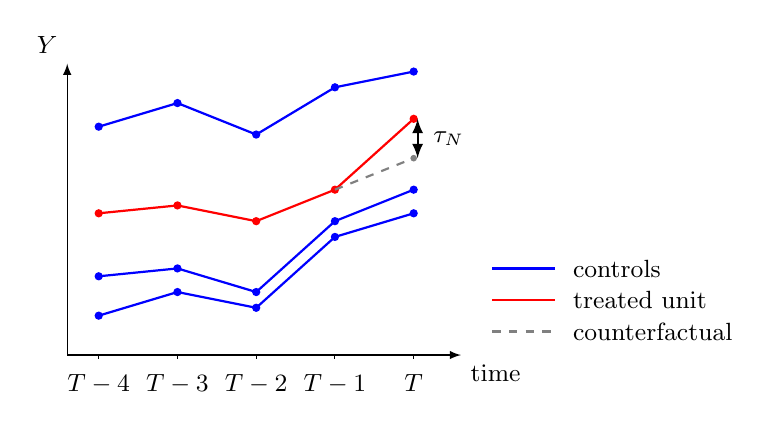
\begin{tikzpicture}[
    >=latex,
    every node/.style={font=\small}
  ]

    % Axes ---------------------------------------------------------
    \draw[->] (0.6,0.3) -- (5.6,0.3) node[below right] {time};
    \draw[->] (0.6,0.3) -- (0.6,4.0) node[above left] {$Y$};

    % Tick marks on time axis
    \foreach \x/\lab in {1/{T-4}, 2/{T-3}, 3/{T-2}, 4/{T-1}, 5/{T}}{
  \draw (\x,0.3) -- (\x,0.25) node[below=2pt] {$\lab$};
}



    % Control trajectories (blue) ----------------------------------
    \draw[blue,thick]
      (1,3.2) -- (2,3.5) -- (3,3.1) -- (4,3.7) -- (5,3.9);
    \foreach \x/\y in {1/3.2,2/3.5,3/3.1,4/3.7,5/3.9}
      \fill[blue] (\x,\y) circle (1.5pt);

    \draw[blue,thick]
      (1,1.3) -- (2,1.4) -- (3,1.1) -- (4,2.0) -- (5,2.4);
    \foreach \x/\y in {1/1.3,2/1.4,3/1.1,4/2.0,5/2.4}
      \fill[blue] (\x,\y) circle (1.5pt);

    \draw[blue,thick]
      (1,0.8) -- (2,1.1) -- (3,0.9) -- (4,1.8) -- (5,2.1);
    \foreach \x/\y in {1/0.8,2/1.1,3/0.9,4/1.8,5/2.1}
      \fill[blue] (\x,\y) circle (1.5pt);

    % Treated trajectory (red) -------------------------------------
    \draw[red,thick]
      (1,2.1) -- (2,2.2) -- (3,2.0) -- (4,2.4) -- (5,3.3);
    \foreach \x/\y in {1/2.1,2/2.2,3/2.0,4/2.4,5/3.3}
      \fill[red] (\x,\y) circle (1.5pt);

    % Counterfactual extension (dashed grey) -----------------------
    \draw[gray,dashed,thick]
      (4,2.4) -- (5,2.8);
    \fill[gray] (5,2.8) circle (1.2pt);

    % Estimand arrow -----------------------------------------------
    \draw[<->,thick]
      (5.05,2.8) -- (5.05,3.3)
      node[midway,right=2pt] {\small $\tau_N$};

    % Legend on the right ------------------------------------------
    \draw[blue,thick] (6.0,1.4) -- (6.8,1.4);
    \node[anchor=west] at (6.9,1.4) {controls};

    \draw[red,thick] (6.0,1.0) -- (6.8,1.0);
    \node[anchor=west] at (6.9,1.0) {treated unit};

    \draw[gray,dashed,thick] (6.0,0.6) -- (6.8,0.6);
    \node[anchor=west] at (6.9,0.6) {counterfactual};

  \end{tikzpicture}
  \caption{} \label{fig:convex_hull}
\end{figure}

\subsection{Convex Hull}
As with DiD, we would like to impute the missing value for $Y_{NT}(0)$. To this end, we make the following assumption.
\begin{assumption}[Convex Hull]\label{ass:convex_hull}
There exist weights $(w_1,\dots,w_{N-1})$ with $w_i \ge 0$ and
$\sum_{i=1}^{N-1} w_i = 1$ such that the untreated potential outcomes of
the treated unit $N$ lie in the convex hull of the control units, i.e., 
\[
  Y_{Nt}(0) = \sum_{i=1}^{N-1} w_i\, Y_{it}(0),
  \qquad t = 1,\ldots,T.
\]
\end{assumption}
Assumption~\ref{ass:convex_hull} states that $Y_{Nt}(0)$ is a \emph{time-invariant}
weighted average of $\{Y_{it}(0)\}_{i=1}^{N-1}$: the same weight vector
$w = (w_1,\dots,w_{N-1})$ links unit $N$ to the donor units in every period.
This encodes a stable structural relationship between the treated unit and the
controls over time.

The constraints $w_i \ge 0$ and $\sum_{i=1}^{N-1} w_i = 1$ restrict the
synthetic control to be an \emph{interpolation} of existing control units
rather than an extrapolation. In particular, the synthetic path
$\sum_{i=1}^{N-1} w_i Y_{it}(0)$ remains inside the convex hull of the control
trajectories; see Figure~\ref{fig:extrapolation_interpolation}. As synthetic control is foremost a prediction method (we predict a single unit, compared to averages), avoiding extrapolation is particularly important (recall OLS). For example, if all control regions have unemployment rates between $5\%$ and $10\%$, an unconstrained regression could fit the pre-treatment data using large
(negative) weights and predict a counterfactual of $20\%$, while the convex-combination restriction forces the synthetic control to remain in the plausible range $[5\%,10\%]$.


\begin{figure}[htbp]
  \centering
  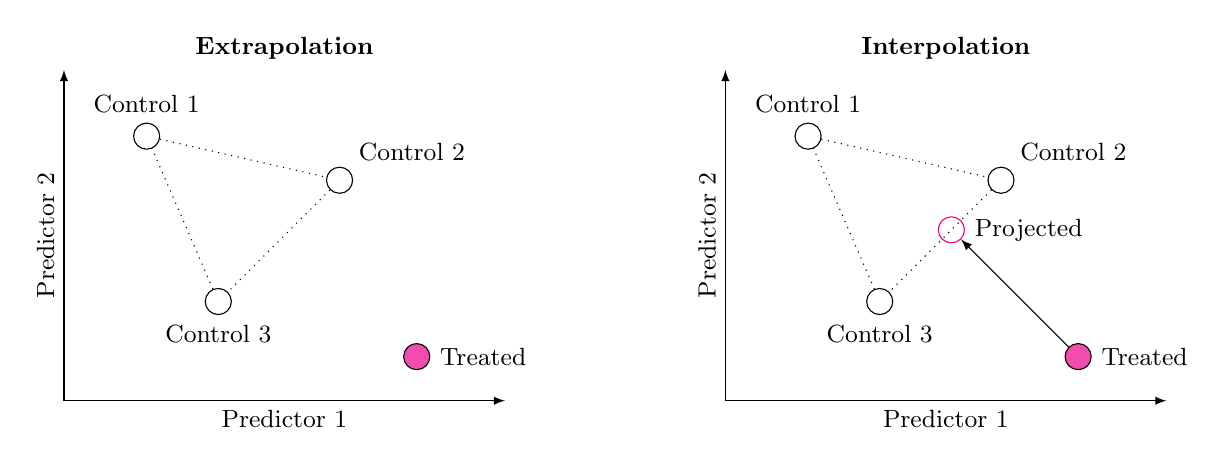
\begin{tikzpicture}[
    >=latex,
    scale=1.4,
    every node/.style={font=\small},
    control/.style={draw, circle, minimum size=5pt},
    treated/.style={draw, circle, fill=magenta!70, minimum size=5pt},
    cftreated/.style={draw=magenta, circle, minimum size=5pt}
  ]

  % \node[below]        at (2,-0.2)   {Time};
  %   \node[rotate=90]    at (-0.2,1.5) {Average Outcome};

    %------------------ Left panel: Extrapolation ------------------%
    \begin{scope}[xshift=0cm]
      % Axes
      \draw[->] (0,0) -- (4,0) node[midway, below] {Predictor 1};
      \draw[->] (0,0) -- (0,3) node[midway, above, rotate=90] {Predictor 2};

      % Title
      \node[font=\small\bfseries] at (2,3.2) {Extrapolation};

      % Controls
       \node[control,label=above:{Control 1}] (c1) at (0.75,2.4) {};
      \node[control,label=above right:{Control 2}] (c2) at (2.5,2.0) {};
      \node[control,label=below:{Control 3}] (c3) at (1.4,0.9) {};

      % Treated (outside convex hull)
      \node[treated,label=right:{Treated}] (tr) at (3.2,0.4) {};

      % % Lines showing extrapolation
      % \draw[thin] (c1) -- (tr);
      % \draw[thin] (c2) -- (tr);
      % \draw[thin] (c3) -- (tr);

      % Convex hull of controls
      \draw[dotted] (c1) -- (c2) -- (c3) -- (c1) -- cycle;

      % Annotation
      % \node[align=center,anchor=north west] at (-0.2,0.3)
      %   {Treated unit lies outside\\ convex hull of controls};
    \end{scope}

    %------------------ Right panel: Interpolation -----------------%
    \begin{scope}[xshift=6cm]
      % Axes
      \draw[->] (0,0) -- (4,0) node[midway, below] {Predictor 1};
      \draw[->] (0,0) -- (0,3) node[midway, above, rotate=90] {Predictor 2};

      % Title
      \node[font=\small\bfseries] at (2,3.2) {Interpolation};

      % Controls
     \node[control,label=above:{Control 1}] (c1) at (0.75,2.4) {};
      \node[control,label=above right:{Control 2}] (c2) at (2.5,2.0) {};
      \node[control,label=below:{Control 3}] (c3) at (1.4,0.9) {};

      % Treated (outside convex hull)
      \node[treated,label=right:{Treated}] (tr) at (3.2,0.4) {};
     \node[cftreated,label= right:{Projected}] (cf) at (2.05,1.55) {};
      % % Lines showing extrapolation
      \draw[->] (tr) -- (cf);
      % \draw[thin] (c2) -- (tr);
      % \draw[thin] (c3) -- (tr);

      % Convex hull of controls
      \draw[dotted] (c1) -- (c2) -- (c3) -- (c1) -- cycle;

      % Annotation
      % \node[align=center,anchor=north west] at (-0.2,0.3)
      %   {Treated unit lies outside\\ convex hull of controls};
    \end{scope}

  \end{tikzpicture}
  \caption{Extrapolation (left) predicts the treatment. Interpolation (right) predicts the treatment and projects it to the convex hull of controls.} \label{fig:extrapolation_interpolation}
\end{figure}

In practice, we fit
\begin{equation}\label{eq:sc_opt_scalar}
  \hat{\mathbf w}
  =
  \arg\min_{\mathbf w}
  \sum_{t=1}^{T-1}
  \left(
    Y_{Nt} - \sum_{i=1}^{N-1} w_i Y_{it}
  \right)^{2}
  \quad\text{subject to}\quad
  \sum_{i=1}^{N-1} w_i = 1,\; w_i \ge 0 \ \forall i,
\end{equation}
and estimate $\widehat Y_{NT}(0) = \sum_{i=1}^{N-1} \hat w_i Y_{iT}$. We then set 
\[
    \hat \tau_N = Y_{NT} - \widehat Y_{NT}(0).
\]
To obtain a good fit this usually requires long, stable pre-treatment trajectories.

\begin{remark}
  Throughout this section we implicitly assume \emph{no spillover effects}:
  treatment of unit $N$ does not affect the outcomes of the control units.
  This assumption is particularly important for synthetic control, since the
  control units are used to construct the counterfactual trajectory for the
  treated unit over many periods. If treatment spills over to the donor pool,
  the synthetic control will no longer represent an untreated path.
\end{remark}

\subsection{Model-Based Justifications}
Assumption~\ref{ass:convex_hull} may look intuitive, but it might be hard to justify. \citet{abadie2010synthetic} provide two models that satisfy the convex hull assumption
\begin{itemize}
    \item \textbf{Factor Model}: 
    \[
        Y_{it}(0) = \gamma_t + \delta_t^\top X_i + \xi_t^\top U_i + \varepsilon_{it},
    \]
    \begin{itemize}
        \item $X_i$ are observed unit-level covariates,
        \item $U_i$ are unobserved time-invariant factors,
        \item Generalization of the linear two-way fixed effects model,
        \item Assumption: exist weights $(w_1,\dots,w_{N-1})$ with $w_i \ge 0$, $\sum_{i=1}^{N-1} w_i = 1$ such that $\sum_{i=1}^{N-1} w_i X_i = X_N, 
  \sum_{i=1}^{N-1} w_i U_i = U_N$.
    \end{itemize}
    \item \textbf{Autoregressive Model}:
    \begin{align*}
            Y_{it}(0) &= \rho_t Y_{i,t-1}(0) + \delta_t^\top X_{it} + \varepsilon_{it}, \\
            X_{it}    &= \lambda_{t-1} Y_{i,t-1}(0) + \Delta_{t-1} X_{i,t-1} + \nu_{it},
    \end{align*}
    \begin{itemize}
        \item Time-varying covariates,
        \item Past outcomes can affect current treatment.
        \item No unobserved time-invariant confounders.
    \end{itemize}
\end{itemize}

\subsection{Inference}

We discuss two methods for inference.

\subsubsection{Placebo Tests}
Our aim is to test $H_0: Y_{NT}(1) = Y_{NT}(0)$ and derive a confidence interval.
To this end, we construct placebo effects for each control unit $j=1,\dots,N-1$:
\begin{itemize}
    \item Pick a unit $j < N$ and treat it as the treated unit,
    \item Fit the synthetic control estimate to obtain $\widehat Y_{jt}(0)$ (include treated unit $i=N$),
    \item Calculate $\hat \tau_N = Y_{jT} - \widehat Y_{jT}(0)$.
\end{itemize}
We do this for every unit $j = 1, \ldots, N$. Assuming that $\{\hat \tau_j\}_{j=1}^{N}$ are exchangeable, we can calculate the (two-sided) permutation $p$-value 
\[
  p
  = \frac{1}{(N-1)+1}
    \Biggl(
      1 + \sum_{j=1}^{N-1} \mathbf{1}\bigl\{|\hat\tau_j|\ge |\hat\tau_N|\bigr\}
    \Biggr).
\]

\begin{remark}
    Assuming that $\{\hat\tau_j\}_{j=1}^N$ are \emph{exchangeable} means that, under
$H_0 : Y_{NT}(1)=Y_{NT}(0)$, the joint distribution of the effects does not
depend on which unit is labeled as ``treated''. Formally, for any permutation
$\pi$ of $\{1,\dots,N\}$,
\[
  (\hat\tau_1,\dots,\hat\tau_N)
  \overset{d}{=} (\hat\tau_{\pi(1)},\dots,\hat\tau_{\pi(N)}).
\]
It also means that the marginals are the same (identically distributed), which can be questionable.
\end{remark}

As always, once we know how to calculate p-values, we can invert them to obtain a confidence interval. Let $H_0: Y_{NT}(1) = Y_{NT}(0) + \tau_0$ and set 
\[
    \hat \tau_N(\tau_0) = (Y_{NT} - \tau_0) - \widehat Y_{NT}(0).
\]
The confidence interval will then consist of all $\tau_0$ for which we don't reject the null.
Note that this method of inference requires a large $N$ to be powerful.


\subsubsection{Variance}
One can assume that $Y_{NT} = Y_{NT}(1)$ is fixed and the only uncertainty arises from the estimation of $Y_{NT}(0)$, using noisy
control trajectories \citep{doudchenko2016balancing}. A simple design-based variance estimator treats the
placebo effects as draws from the baseline noise distribution and sets
\[
  \widehat{\Var}(\hat\tau_N)
  = \frac{1}{N-1}\sum_{j=1}^{N-1} \hat\tau_j^{\,2}.
\]


\subsubsection{Diagnostics}
\begin{itemize}
    \item Look at pre-treatment fit of treated and placebo units.
    \item Compare the RMSE before and after treatment for placebo units.
\end{itemize}





\subsection{Extensions}
\begin{itemize}
    \item \textbf{Adding Covariates}: Define $  Z_i = \begin{pmatrix} Y_i \\[0.2em] X_i \end{pmatrix},
      \quad
      Y_i = (Y_{i1},\dots,Y_{i,T-1})^\top,
      \quad
      X_i = (X_{i1}^\top,\dots,X_{i,T-1}^\top)^\top $ and solve

  \[
    \hat w
    =
    \arg\min_{w}
    \Bigl(
      Z_N - \sum_{i=1}^{N-1} w_i Z_i
    \Bigr)^{\!\top}
    \hat \Sigma_Z^{-1}
    \Bigl(
      Z_N - \sum_{i=1}^{N-1} w_i Z_i
    \Bigr)
  \]
  \[
    \text{subject to}\qquad
    \sum_{i=1}^{N-1} w_i = 1,
    \qquad
    w_i \ge 0 \ \text{for } i=1,\dots,N-1,
  \]
  where $\hat \Sigma_Z$ is a covariance (or weighting) matrix for the components of
  $Z_i$.

    \item \textbf{Bias Correction}: Similar to the bias-corrected matching estimator, we can adjust for possible bias due to poor pre-treatment fit, see \cite{ben2021augmented}.
    \item \textbf{Regularization}: Standard synthetic control method tends to overfit. \citet{abadie2021penalized} propose additional regularization.
 \[
    \arg\min_{w}
    \left\{
      \underbrace{
        \sum_{t=1}^{T-1}
        \left(
          Y_{Nt} - \sum_{i=1}^{N-1} w_i Y_{it}
        \right)^2
      }_{\text{component-wise fit}}
      +
      \lambda\,
      \underbrace{
        \sum_{i=1}^{N-1} w_i
        \sum_{t=1}^{T-1}
        \bigl(Y_{Nt} - Y_{it}\bigr)^2
      }_{\text{aggregate fit}}
    \right\}
  \]
    \begin{itemize}
    \item $\lambda \to 0$: synthetic control.
    \item $\lambda \to \infty$: nearest neighbor matching.
  \end{itemize}
  \item \textbf{Staggered Adoption}: Synthetic control can be extended to staggered adoption, see \citet{ben2022synthetic}.
    \item \textbf{Matrix Completion}: Synthetic control is essentially just a restricted weighted regression where we are interest in filling in the missing data in the following matrix (assuming $T_1$ post-time periods and $N_1$ treated units).
    \[
\mathbf Y(0)
=
\left[
\begin{array}{ccc|ccc}
Y_{1,1}   & \cdots & Y_{1,T-1}   & Y_{1,T}   & \cdots & Y_{1,T+T_1} \\
\vdots    &        & \vdots      & \vdots    &        & \vdots    \\
\vdots    & \ddots & \vdots      & \vdots    & \ddots & \vdots    \\
Y_{N,1}   & \cdots & Y_{N,T-1}   & Y_{N,T}   & \cdots & Y_{N,T+T_1} \\
\vdots    &        & \vdots      & \vdots    &        & \vdots    \\
Y_{N+N_1,1} & \cdots & Y_{N+N_1,T-1} & ?      & \cdots & ?         \\
\end{array}
\right].
\]
    Weighted regression seems to be a strong parametric assumption. Instead, \citet{athey2021matrix} propose to view this as a matrix completion problem, assuming an underlying low-rank structure.
\end{itemize}





\subsection{When to use Synthetic Control}
\begin{itemize}
    \item Use when you have a large donor pool of control units and long pre-treatment histories.
    \item You are interested in the effect of a single or a small number of treated units
    \item Obtain individual effects, lack of external validity
\end{itemize}









\endgroup

\newpage

\bibliography{references}


\end{document}
